\documentclass{standalone}
\usepackage{tikz}
\usetikzlibrary{patterns, positioning}


\begin{document}
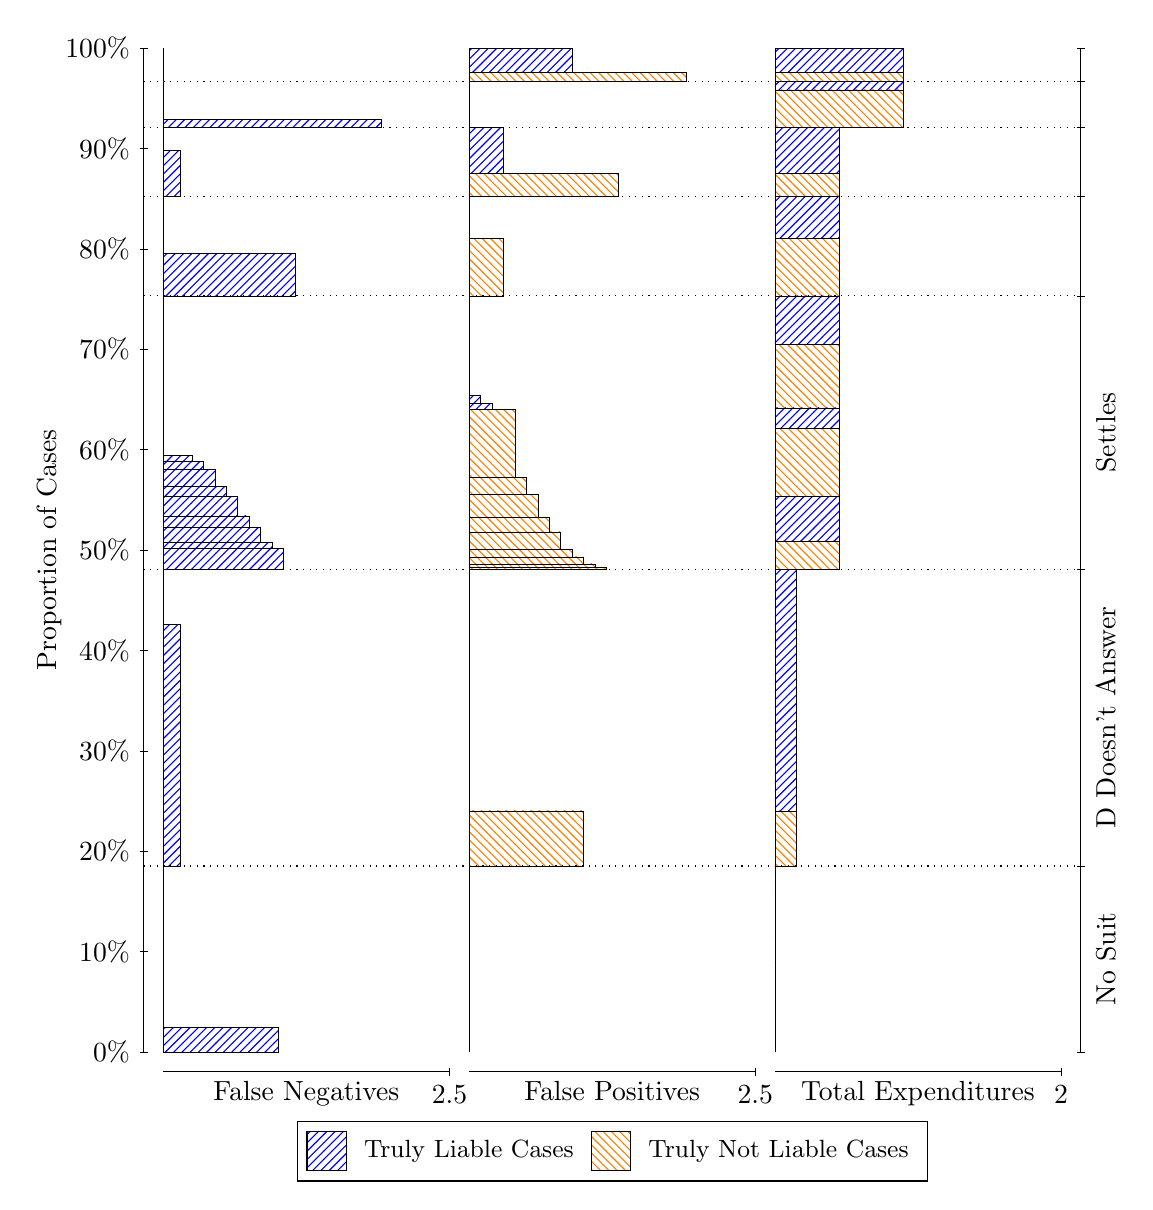
\begin{tikzpicture}
\draw[black, very thin] (1.5,1.75) -- (1.5,14.5);
\node[rotate=90, text=black, anchor=center] at (0.3, 8.125) {Proportion of Cases};
\draw[black, very thin] (1.45,1.75) -- (1.55,1.75);
\node[text=black, anchor=east] at (1.45, 1.75) {0\%};
\draw[black, very thin] (1.45,3.025) -- (1.55,3.025);
\node[text=black, anchor=east] at (1.45, 3.025) {10\%};
\draw[black, very thin] (1.45,4.3) -- (1.55,4.3);
\node[text=black, anchor=east] at (1.45, 4.3) {20\%};
\draw[black, very thin] (1.45,5.575) -- (1.55,5.575);
\node[text=black, anchor=east] at (1.45, 5.575) {30\%};
\draw[black, very thin] (1.45,6.85) -- (1.55,6.85);
\node[text=black, anchor=east] at (1.45, 6.85) {40\%};
\draw[black, very thin] (1.45,8.125) -- (1.55,8.125);
\node[text=black, anchor=east] at (1.45, 8.125) {50\%};
\draw[black, very thin] (1.45,9.4) -- (1.55,9.4);
\node[text=black, anchor=east] at (1.45, 9.4) {60\%};
\draw[black, very thin] (1.45,10.675) -- (1.55,10.675);
\node[text=black, anchor=east] at (1.45, 10.675) {70\%};
\draw[black, very thin] (1.45,11.95) -- (1.55,11.95);
\node[text=black, anchor=east] at (1.45, 11.95) {80\%};
\draw[black, very thin] (1.45,13.225) -- (1.55,13.225);
\node[text=black, anchor=east] at (1.45, 13.225) {90\%};
\draw[black, very thin] (1.45,14.5) -- (1.55,14.5);
\node[text=black, anchor=east] at (1.45, 14.5) {100\%};

\draw[black, very thin] (13.4,1.75) -- (13.4,14.5);
\draw[black, very thin] (13.35,1.75) -- (13.45,1.75);
\node[anchor=west] at (13.35, 1.75) {};
\draw[black, very thin] (13.35,4.1113) -- (13.45,4.1113);
\node[anchor=west] at (13.35, 4.1113) {};
\draw[black, very thin] (13.35,7.8823) -- (13.45,7.8823);
\node[anchor=west] at (13.35, 7.8823) {};
\draw[black, very thin] (13.35,11.353) -- (13.45,11.353);
\node[anchor=west] at (13.35, 11.353) {};
\draw[black, very thin] (13.35,12.62) -- (13.45,12.62);
\node[anchor=west] at (13.35, 12.62) {};
\draw[black, very thin] (13.35,13.488) -- (13.45,13.488);
\node[anchor=west] at (13.35, 13.488) {};
\draw[black, very thin] (13.35,14.078) -- (13.45,14.078);
\node[anchor=west] at (13.35, 14.078) {};
\draw[black, very thin] (13.35,14.5) -- (13.45,14.5);
\node[anchor=west] at (13.35, 14.5) {};

\draw[black, very thin, pattern color=blue, pattern=north east lines] (1.75,1.75) rectangle (3.2033,2.0664);
\draw[black, very thin, pattern color=orange, pattern=north west lines] (1.75,2.0664) rectangle (1.75,4.1113);
\draw[black, very thin, pattern color=blue, pattern=north east lines] (1.75,4.1113) rectangle (1.968,7.1814);
\draw[black, very thin, pattern color=orange, pattern=north west lines] (1.75,7.1814) rectangle (1.75,7.8823);
\draw[black, very thin, pattern color=blue, pattern=north east lines] (1.75,7.8823) rectangle (3.276,8.1423);
\draw[black, very thin, pattern color=blue, pattern=north east lines] (1.75,8.1423) rectangle (3.1307,8.225);
\draw[black, very thin, pattern color=blue, pattern=north east lines] (1.75,8.225) rectangle (2.9853,8.4075);
\draw[black, very thin, pattern color=blue, pattern=north east lines] (1.75,8.4075) rectangle (2.84,8.5569);
\draw[black, very thin, pattern color=blue, pattern=north east lines] (1.75,8.5569) rectangle (2.6947,8.8108);
\draw[black, very thin, pattern color=blue, pattern=north east lines] (1.75,8.8108) rectangle (2.5493,8.9342);
\draw[black, very thin, pattern color=blue, pattern=north east lines] (1.75,8.9342) rectangle (2.404,9.1466);
\draw[black, very thin, pattern color=blue, pattern=north east lines] (1.75,9.1466) rectangle (2.2587,9.2465);
\draw[black, very thin, pattern color=blue, pattern=north east lines] (1.75,9.2465) rectangle (2.1133,9.3244);
\draw[black, very thin, pattern color=orange, pattern=north west lines] (1.75,9.3244) rectangle (1.75,11.353);
\draw[black, very thin, pattern color=blue, pattern=north east lines] (1.75,11.353) rectangle (3.4213,11.893);
\draw[black, very thin, pattern color=orange, pattern=north west lines] (1.75,11.893) rectangle (1.75,12.62);
\draw[black, very thin, pattern color=blue, pattern=north east lines] (1.75,12.62) rectangle (1.968,13.203);
\draw[black, very thin, pattern color=orange, pattern=north west lines] (1.75,13.203) rectangle (1.75,13.488);
\draw[black, very thin, pattern color=blue, pattern=north east lines] (1.75,13.488) rectangle (4.5113,13.597);
\draw[black, very thin, pattern color=orange, pattern=north west lines] (1.75,13.597) rectangle (1.75,14.078);
\draw[black, very thin, pattern color=orange, pattern=north west lines] (1.75,14.078) rectangle (1.75,14.186);
\draw[black, very thin, pattern color=blue, pattern=north east lines] (1.75,14.186) rectangle (1.75,14.5);
\draw[black, very thin, pattern color=orange, pattern=north west lines] (5.6333,1.75) rectangle (5.6333,3.7949);
\draw[black, very thin, pattern color=blue, pattern=north east lines] (5.6333,3.7949) rectangle (5.6333,4.1113);
\draw[black, very thin, pattern color=orange, pattern=north west lines] (5.6333,4.1113) rectangle (7.0867,4.8122);
\draw[black, very thin, pattern color=blue, pattern=north east lines] (5.6333,4.8122) rectangle (5.6333,7.8823);
\draw[black, very thin, pattern color=orange, pattern=north west lines] (5.6333,7.8823) rectangle (7.3773,7.9075);
\draw[black, very thin, pattern color=orange, pattern=north west lines] (5.6333,7.9075) rectangle (7.232,7.9487);
\draw[black, very thin, pattern color=orange, pattern=north west lines] (5.6333,7.9487) rectangle (7.0867,8.0378);
\draw[black, very thin, pattern color=orange, pattern=north west lines] (5.6333,8.0378) rectangle (6.9413,8.1295);
\draw[black, very thin, pattern color=orange, pattern=north west lines] (5.6333,8.1295) rectangle (6.796,8.3563);
\draw[black, very thin, pattern color=orange, pattern=north west lines] (5.6333,8.3563) rectangle (6.6507,8.5387);
\draw[black, very thin, pattern color=orange, pattern=north west lines] (5.6333,8.5387) rectangle (6.5053,8.8264);
\draw[black, very thin, pattern color=orange, pattern=north west lines] (5.6333,8.8264) rectangle (6.36,9.0476);
\draw[black, very thin, pattern color=orange, pattern=north west lines] (5.6333,9.0476) rectangle (6.2147,9.9112);
\draw[black, very thin, pattern color=blue, pattern=north east lines] (5.6333,9.9112) rectangle (5.924,9.9891);
\draw[black, very thin, pattern color=blue, pattern=north east lines] (5.6333,9.9891) rectangle (5.7787,10.089);
\draw[black, very thin, pattern color=blue, pattern=north east lines] (5.6333,10.089) rectangle (5.6333,11.353);
\draw[black, very thin, pattern color=orange, pattern=north west lines] (5.6333,11.353) rectangle (6.0693,12.08);
\draw[black, very thin, pattern color=blue, pattern=north east lines] (5.6333,12.08) rectangle (5.6333,12.62);
\draw[black, very thin, pattern color=orange, pattern=north west lines] (5.6333,12.62) rectangle (7.5227,12.904);
\draw[black, very thin, pattern color=blue, pattern=north east lines] (5.6333,12.904) rectangle (6.0693,13.488);
\draw[black, very thin, pattern color=orange, pattern=north west lines] (5.6333,13.488) rectangle (5.6333,13.969);
\draw[black, very thin, pattern color=blue, pattern=north east lines] (5.6333,13.969) rectangle (5.6333,14.078);
\draw[black, very thin, pattern color=orange, pattern=north west lines] (5.6333,14.078) rectangle (8.3947,14.186);
\draw[black, very thin, pattern color=blue, pattern=north east lines] (5.6333,14.186) rectangle (6.9413,14.5);
\draw[black, very thin, pattern color=orange, pattern=north west lines] (9.5167,1.75) rectangle (9.5167,3.7949);
\draw[black, very thin, pattern color=blue, pattern=north east lines] (9.5167,3.7949) rectangle (9.5167,4.1113);
\draw[black, very thin, pattern color=orange, pattern=north west lines] (9.5167,4.1113) rectangle (9.7892,4.8122);
\draw[black, very thin, pattern color=blue, pattern=north east lines] (9.5167,4.8122) rectangle (9.7892,7.8823);
\draw[black, very thin, pattern color=orange, pattern=north west lines] (9.5167,7.8823) rectangle (10.334,8.2394);
\draw[black, very thin, pattern color=blue, pattern=north east lines] (9.5167,8.2394) rectangle (10.334,8.8056);
\draw[black, very thin, pattern color=orange, pattern=north west lines] (9.5167,8.8056) rectangle (10.334,9.6692);
\draw[black, very thin, pattern color=blue, pattern=north east lines] (9.5167,9.6692) rectangle (10.334,9.9292);
\draw[black, very thin, pattern color=orange, pattern=north west lines] (9.5167,9.9292) rectangle (10.334,10.737);
\draw[black, very thin, pattern color=blue, pattern=north east lines] (9.5167,10.737) rectangle (10.334,11.353);
\draw[black, very thin, pattern color=orange, pattern=north west lines] (9.5167,11.353) rectangle (10.334,12.08);
\draw[black, very thin, pattern color=blue, pattern=north east lines] (9.5167,12.08) rectangle (10.334,12.62);
\draw[black, very thin, pattern color=orange, pattern=north west lines] (9.5167,12.62) rectangle (10.334,12.904);
\draw[black, very thin, pattern color=blue, pattern=north east lines] (9.5167,12.904) rectangle (10.334,13.488);
\draw[black, very thin, pattern color=orange, pattern=north west lines] (9.5167,13.488) rectangle (11.152,13.969);
\draw[black, very thin, pattern color=blue, pattern=north east lines] (9.5167,13.969) rectangle (11.152,14.078);
\draw[black, very thin, pattern color=orange, pattern=north west lines] (9.5167,14.078) rectangle (11.152,14.186);
\draw[black, very thin, pattern color=blue, pattern=north east lines] (9.5167,14.186) rectangle (11.152,14.5);
\draw[black, dotted] (1.5,4.1113) -- (13.4,4.1113);
\draw[black, dotted] (1.5,7.8823) -- (13.4,7.8823);
\draw[black, dotted] (1.5,11.353) -- (13.4,11.353);
\draw[black, dotted] (1.5,12.62) -- (13.4,12.62);
\draw[black, dotted] (1.5,13.488) -- (13.4,13.488);
\draw[black, dotted] (1.5,14.078) -- (13.4,14.078);
\draw[black, very thin] (1.75,1.5) -- (5.3833,1.5);
\node[text=black, anchor=north] at (3.5667, 1.5) {False Negatives};
\draw[black, very thin] (5.3833,1.45) -- (5.3833,1.55);
\node[text=black, anchor=north] at (5.3833, 1.45) {2.5};

\draw[black, very thin] (5.6333,1.5) -- (9.2667,1.5);
\node[text=black, anchor=north] at (7.45, 1.5) {False Positives};
\draw[black, very thin] (9.2667,1.45) -- (9.2667,1.55);
\node[text=black, anchor=north] at (9.2667, 1.45) {2.5};

\draw[black, very thin] (9.5167,1.5) -- (13.15,1.5);
\node[text=black, anchor=north] at (11.333, 1.5) {Total Expenditures};
\draw[black, very thin] (13.15,1.45) -- (13.15,1.55);
\node[text=black, anchor=north] at (13.15, 1.45) {2};

\node[text=black, centered, rotate=90] at (13.72, 2.9306) {No Suit};
\node[text=black, centered, rotate=90] at (13.72, 5.9968) {D Doesn't Answer};
\node[text=black, centered, rotate=90] at (13.72, 9.6178) {Settles};





\draw (7.449999999999999,1.5) node[draw=none] (baseCoordinate) {};
\begin{scope}[align=center]
        \matrix[scale=0.5, draw=black, below=0.5cm of baseCoordinate, nodes={draw}, column sep=0.1cm]{
            \node[rectangle, draw, minimum width=0.5cm, minimum height=0.5cm, pattern color=blue, pattern=north east lines] {}; &
            \node[draw=none, font=\small, text=black] (B) {Truly Liable Cases}; &
            \node[rectangle, draw, minimum width=0.5cm, minimum height=0.5cm, pattern color=orange, pattern=north west lines] {}; &
            \node[draw=none, font=\small, text=black] (B) {Truly Not Liable Cases}; \\
            };
\end{scope}

\end{tikzpicture}
\end{document}